\chapter*{Preliminary Concepts}
\section{Interpretable Sequential Decision Making}
\subsection{What is Sequential Decision Making?}

In this manuscript we are mostly interested in sequential decision making. Humans engage in sequential decision making in all aspects of life. In medicine, doctors have to decide when to use chemotherapy next based on the patient's current health in order to heal (cite). In agriculture, agronomists have to decide when to fertilize next based on the current soil and weather conditions in order to maximize plant growth (cite). 
In automotive, the auto-pilot system has to decide how to steer the wheel next based on lidar sensors in order to maintain a safe trajectory (cite). In video games, a bot decides what attack to throw next based on the player's and its own state in order to provide the best entertainment (cite).
Those sequential decision making processes exhibits key similarities: an agent takes actions based on some current information to achieve some goal.
As computer scientists, we ought to design computer programs (cite) that can help humans during those sequential decision making processes. 
For example, a doctor could benefit from a program that would recommend the ``best'' treatment given the patient's state. 
Machine learning arlgortihms (cite) output such helpful programs. Every day, hundreds of new machine learning algorithms are published\footnote{\url{https://arxiv.org/list/cs.LG/pastweek?skip=0&show=2000}}. While most of those scientific articles focus on finding the ``best'' program possible, not many work make sure that their recommendations can be understood by humans.
Deep learning algorithms (cite) are machine learing algorithms that train neural networks because they can leverage the backpropagation algorithm (cite) for efficient learning from example data, e.g. records of patients.
Next, we describe the notion of interpretability that is key to ensure safe deployment of cpmputer programs trained with machine learning in critical sectors like medicine. 

\begin{figure}[htbp]
    \centering
    \begin{tikzpicture}[
        node distance=2.5cm,
        auto,
        thick,
        state/.style={circle, draw, fill=blue!20, minimum size=1.5cm, text centered},
        environment/.style={rectangle, draw, dashed, fill=blue!10, rounded corners, minimum width=4cm, minimum height=2cm, text centered},
        agent/.style={rectangle, draw, fill=orange!20, rounded corners, minimum width=2cm, minimum height=1.5cm, text centered},
        robot/.style={rectangle, draw, fill=green!20, rounded corners, minimum width=2cm, minimum height=1.5cm, text centered},
        decision_box/.style={rectangle, draw, dashed, fill=gray!10, minimum width=7.5cm, minimum height=3cm, text centered},
        arrow/.style={->, thick, bend left=15},
        arrow_decision/.style={->, dashed, bend left=15}
    ]
        
        % Decision Making Box
        \node[decision_box] (decision_box) at (0.3,3.4) {};
        \node at (0.3,4.5) {\small{Decision Making}};
        
        % Robot (AI)
        \node[robot] (robot) at (-2.1,3.2) {
            \begin{minipage}{1.5cm}
                \centering
                \includesvg[width=0.4cm]{images/images_intro/robot-svgrepo-com.svg}\\
                \small{Computer program}
            \end{minipage}
        };
        
        % Doctor
        \node[agent] (doctor) at (2.5,3.2) {
            \begin{minipage}{1.5cm}
                \centering
                \includesvg[width=0.4cm]{images/images_intro/doctor-with-stethoscope-svgrepo-com.svg}\\
                \small{Doctor}
            \end{minipage}
        };
        
        % Environment (Patient)
        \node[environment] (environment) at (0,-0.5) {
            \begin{minipage}{2cm}
                \centering
                \includesvg[width=0.8cm]{images/images_intro/patient-4.svg}\\
                \small{Cancer patient}
            \end{minipage}
        };
        
        % Arrows
        \draw[arrow] (environment) to[bend left=30] node[left] {
            \begin{minipage}{2cm}
                \centering
                \includesvg[width=0.4cm]{images/images_intro/patient-clipboard-svgrepo-com.svg}\\
                \small{Updated health status}
            \end{minipage}
        } (robot);
        \draw[arrow_decision] (robot) to node[above] {\small{Recommends}} (doctor);
        \draw[arrow_decision] (doctor) to node[below] {\small{Interprets}} (robot);

        \draw[arrow] (doctor) to[bend left=30] node[right] {
            \begin{minipage}{1.5cm}
                \centering
                \includesvg[width=0.5cm]{images/images_intro/syringe-svgrepo-com.svg}\\
                \small{Administrate chemo}
            \end{minipage}
        } (environment);
        
    \end{tikzpicture}
    \caption{Sequential decision making in cancer treatment. The AI system is informed by the patient's current state (tumor size, blood counts, etc.) and makes a recommendation to the doctor, who administers the chemotherapy directly to the patient. The patient's state is then updated, and this cycle repeats over time.}
    \label{fig:cancer-treatment-sdm}
\end{figure}

\begin{figure}[htbp]
    \centering
    \begin{tikzpicture}[
        node distance=2.5cm,
        auto,
        thick,
        state/.style={circle, draw, fill=blue!20, minimum size=1.5cm, text centered},
        environment/.style={rectangle, draw, dashed, fill=blue!10, rounded corners, minimum width=4cm, minimum height=2cm, text centered},
        agent/.style={rectangle, draw, fill=orange!20, rounded corners, minimum width=2cm, minimum height=1.5cm, text centered},
        robot/.style={rectangle, draw, fill=black!20, rounded corners, minimum width=2cm, minimum height=1.5cm, text centered},
        ml/.style={circle, draw, fill=purple!20, minimum width=2cm, minimum height=1cm, text centered},
        decision_box/.style={rectangle, draw, dashed, fill=gray!10, minimum width=7.5cm, minimum height=3cm, text centered},
        arrow/.style={->, thick, bend left=15},
        arrow_decision/.style={->, dashed, bend left=15}
    ]
        
        % Decision Making Box
        \node[decision_box] (decision_box) at (0.3,3.4) {};
        \node at (0.3,4.5) {\small{Decision Making}};
        
        % Robot (AI)
        \node[robot] (robot) at (-2.1,3.2) {
            \begin{minipage}{1.5cm}
                \centering
                \includesvg[width=0.4cm]{images/images_intro/network-mapping-svgrepo-com.svg}\\
                \small{Neural network}
            \end{minipage}
        };
        
        % Doctor
        \node[agent] (doctor) at (2.5,3.2) {
            \begin{minipage}{1.5cm}
                \centering
                \includesvg[width=0.4cm]{images/images_intro/doctor-with-stethoscope-svgrepo-com.svg}\\
                \small{Doctor}
            \end{minipage}
        };
        
        % Machine Learning component
        \node[ml] (ml) at (-7,3) {
            \begin{minipage}{1.8cm}
                \centering
                \includesvg[width=0.4cm]{images/images_intro/gear-file-svgrepo-com.svg}\\
                \small{Machine learning}
            \end{minipage}
        };
        
        % Environment (Patient)
        \node[environment] (environment) at (0,-0.5) {
            \begin{minipage}{2cm}
                \centering
                \includesvg[width=0.8cm]{images/images_intro/patient-4.svg}\\
                \small{Cancer patient}
            \end{minipage}
        };
        
        % Arrows
        \draw[arrow] (environment) to[bend left=30] node[left] {
            \begin{minipage}{2cm}
                \centering
                \includesvg[width=0.5cm]{images/images_intro/patient-clipboard-svgrepo-com.svg}\\
                \small{Updated health status}
            \end{minipage}
        } (robot);
        \draw[arrow_decision] (robot) to node[above] {\small{Recommends}} (doctor);
        \draw[arrow_decision, red] (doctor) to node[below] {\small{Can't interpret}} (robot);
        
        \draw[arrow] (doctor) to[bend left=30] node[right] {
            \begin{minipage}{1.5cm}
                \centering
                \includesvg[width=0.5cm]{images/images_intro/syringe-svgrepo-com.svg}\\
                \small{Administrate chemo}
            \end{minipage}
        } (environment);
        
        % ML learning arrows
        \draw[arrow] (environment) to[bend left=40] node[left] {
            \begin{minipage}{2cm}
                \centering
                \includesvg[width=0.5cm]{images/images_intro/patient-clipboard-svgrepo-com.svg}\\
                \small{Treatment outcomes}
            \end{minipage}
        } (ml);
        \draw[arrow] (ml) to[bend left=20] node[above] {
            \begin{minipage}{1.5cm}
                \centering
                \small{Updates program}
            \end{minipage}
        } (robot);
        
    \end{tikzpicture}
    \caption{Sequential decision making with machine learning in cancer treatment. The ML system learns from treatment outcomes to continuously improve the computer program's recommendations, creating a feedback loop for better patient care over time.}
    \label{fig:cancer-treatment-sdm-ml}
\end{figure}

\subsection{What is Interpretability?}
\begin{figure}[htbp]
    \centering
    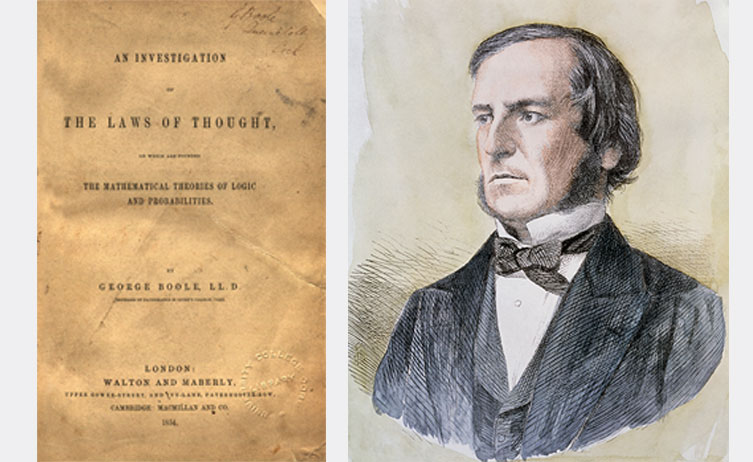
\includegraphics[width=0.5\textwidth]{images/images_intro/gboole.jpg}
    \caption{British logician and philosopher George Boole (1815-1864) next to its book \textit{The Laws of Thoughts} (1854) that is the oldest known record of the word ``interpretability''.}
\end{figure}

Interpretability is a crucial topic in modern science. While computer programs trained with machine learning algorithms have become more and more performing and made their way into our society, they are often black-box: their outputs, e.g., the animals on the image (cite), tokamak control (cite), or even the abstract of your next article (cite), are computed with operations that are too complex for humans to fully understand.
Indeed most of recent machine learning breakthroughs are obtained by training very large programs like neural networks (cite) which are black-box by definition since they perform sometimes millions of operations on their inputs.
Originally, the etymology of ``interpretability'' is the Latin ``interpretabilis'' meaning ``that can be understood and explained''.

According to the Oxford English dictionary, the first recorded use of the english word ``interpretability'' dates back to 1854 when the british logician George Boole (figure) described the addition of concepts:

\begin{displaycquote}[pp.~48]{(cite)}
I would remark in the first place that the generality of a method in Logic
must very much depend upon the generality of its elementary processes and laws.
We have, for instance, in the previous sections of this work investigated, among
other things, the laws of that logical process of addition which is symbolized by
the sign +. Now those laws have been determined from the study of instances,
in all of which it has been a necessary condition, that the classes or things added
together in thought should be mutually exclusive. The expression x + y seems
indeed uninterpretable, unless it be assumed that the things represented by x
and the things represented by y are entirely separate; that they embrace no
individuals in common. And conditions analogous to this have been involved
in those acts of conception from the study of which the laws of the other
symbolical operations have been ascertained. The question then arises, whether
it is necessary to restrict the application of these symbolical laws and processes
by the same conditions of interpretability under which the knowledge of them
was obtained. If such restriction is necessary, it is manifest that no such thing
as a general method in Logic is possible. On the other hand, if such restriction
is unnecessary, in what light are we to contemplate processes which appear to
be uninterpretable in that sphere of thought which they are designed to aid?
\end{displaycquote}
What is remarkable is that the supposedly first recored occurrence of ``interpretability'' was in the context of (pre-)computer science. Boole asked: \textit{when can we meaningfully apply formal mathematical operations beyond the specific conditions under which we understand them?}
In Boole's era, the concern was whether logical operations like addition could be applied outside their original interpretable contexts—where symbols and their sum represent concepts that humans can understand, e.g. red + apples = red apples. Today, we face an analogous dilemma with machine learning algorithms: neural networks learn complex un-intellegible combinations of inputs (representations), but we often deploy them in contexts where operations should be unerstood by humans, e.g., in medicine. 

Circling back to our cancer treatment example, we would ideally want doctors to have access to computer programs that can recommend ``good'' treatments and which operations can be understood. Those two aspects of machine learning models--performance and interpretability--often compromise; highly performing models like neural networks are often less interpretable and vice-versa (cite).
However, we will observe later on that aiming for interpretability is not necessarily always constraining but can be a quite positive bias for performances in some domains like video games.
Interestingly, one of the key challenges of doing research in interpretability is the lack of formalism; there is no definition of what is an interpretable compute program such as an MDP policy. Throughout this manuscript we make the hypothesis that interpretability is the (space and time) complexity of a program (cite) and hence mostly focus on decision trees (low complexity) (cite) and neural networks (high complexity).  
Despite this lack of formalism the necessity of deploying interpretable models has sparked many works that we present next.
\subsection{What are existing approaches for learning interpretable programs?}
Techniques associated with interpretability in machine learning are either global or local. 
Global methods output a whole model that is interpretable while local approaches LIME FI (cite) output explanations of parts of the model such as how the model considers each part of a single specific input.
\begin{figure}[htbp]
    \centering
    \begin{subfigure}[b]{0.32\textwidth}
        \centering
        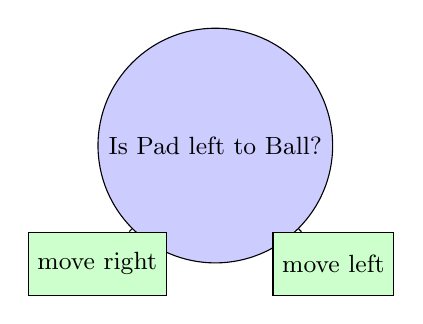
\begin{tikzpicture}[
            level/.style={sibling distance=30mm/#1},
            every node/.style={circle, draw, fill=blue!20, minimum size=1.5cm, text centered, font=\small},
            leaf/.style={rectangle, draw, fill=green!20, minimum width=1.5cm, minimum height=0.8cm, text centered, font=\small}
        ]
        \node {Is Pad left to Ball?}
            child {
                node[leaf] {move right}
            }
            child {
                node[leaf] {move left}  
            };
        \end{tikzpicture}
        \caption{Decision tree}
        \label{fig:decision-tree}
    \end{subfigure}
    \hfill
    \begin{subfigure}[b]{0.32\textwidth}
        \centering
        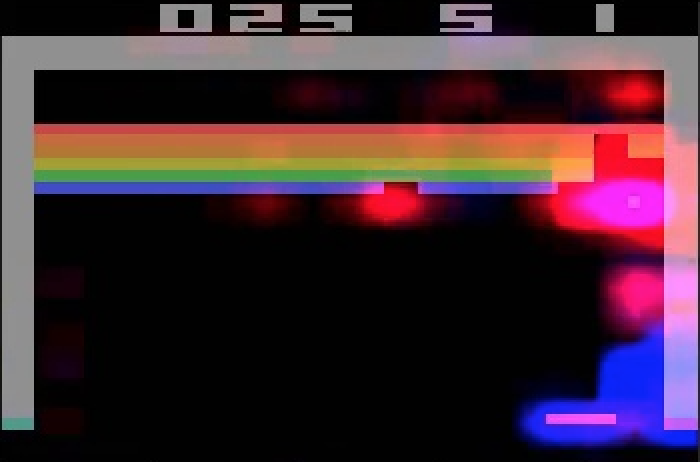
\includegraphics[width=\textwidth]{images/images_intro/breakout_control.png}
        \caption{Placeholder 1}
        \label{fig:placeholder1}
    \end{subfigure}
    \hfill
    \begin{subfigure}[b]{0.32\textwidth}
        \centering
        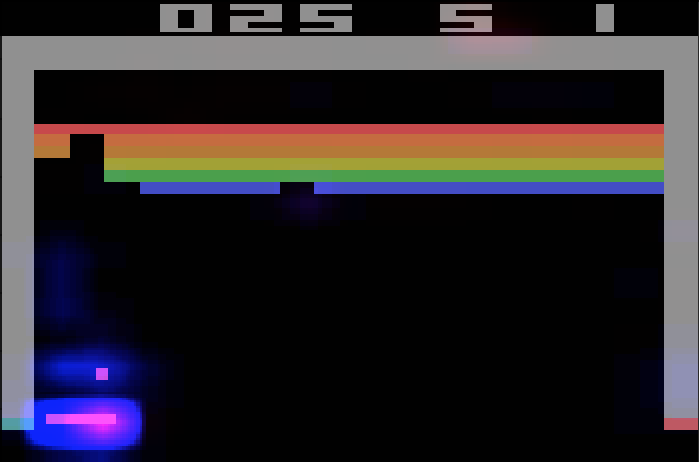
\includegraphics[width=\textwidth]{images/images_intro/breakout_reflect_bp.png}
        \caption{Placeholder 3}
        \label{fig:placeholder3}
    \end{subfigure}
    \caption{Different approaches for learning interpretable programs. (a) Decision tree showing simple binary decision making, (b-d) Additional interpretable model representations.}
    \label{fig:interpretable-approaches}
\end{figure}

(table)
\begin{table}[htbp]
    \centering
    \caption{Related work in \textit{global} interpretable machine learning following the direct/indirect classification. Each class is further divided into the type of interpretable model they output. Methods specific to supervised learning are colored in {\color{red} red} and methods specific to reinforcement learning are in {\color{blue} blue}}\label{tab:related-work}
    \begin{tabular}{|cccc|cccc|}
        \toprule
        \multicolumn{4}{|c|}{\textbf{Direct}} &
        \multicolumn{4}{|c|}{\textbf{indirect}} \\
        \midrule
        (cite) &(cite) &(cite) &(cite) &(cite) &(cite) &(cite) &(cite) \\
        (cite) &(cite) &(cite) &(cite) &(cite) &(cite) &(cite) &(cite) \\
        (cite) &(cite) &(cite) &(cite) &(cite) &(cite) &(cite) &(cite) \\
        \bottomrule
    \end{tabular}
\end{table}
Inside global interpretable machine learning, approaches are either direct or indirect. Direct algorithms like decision tree induction (cite) are algorithms that directly search a space of interpretable models. On the other hand are indirect methods--sometimes called post-hoc--that attempt to interpret some parts of non-interpretable model (cite).
In Table~\ref{tab:related-work} we present both supervised and reinforcement learning works on global interpretability. For reviews of other aspects of interpretable machine learning such as understaning not only the model but also the learning process or on local approaches see (cite). 


An ideal solution to interpretability would be to have global methods that outputs highl performing models. However there is no definite answer as to which is better between direct and indirect algorithms.
\begin{figure}[htbp]
    \centering
    \begin{tikzpicture}[
        node distance=2.5cm,
        auto,
        thick,
        state/.style={circle, draw, fill=blue!20, minimum size=1.5cm, text centered},
        environment/.style={rectangle, draw, dashed, fill=blue!10, rounded corners, minimum width=4cm, minimum height=2cm, text centered},
        agent/.style={rectangle, draw, fill=orange!20, rounded corners, minimum width=2cm, minimum height=1.5cm, text centered},
        robot/.style={rectangle, draw, fill=green!20, rounded corners, minimum width=2cm, minimum height=1.5cm, text centered},
        ml/.style={circle, draw, fill=purple!20, minimum width=2cm, minimum height=1cm, text centered},
        decision_box/.style={rectangle, draw, dashed, fill=gray!10, minimum width=7.5cm, minimum height=3cm, text centered},
        arrow/.style={->, thick, bend left=15},
        arrow_decision/.style={->, dashed, bend left=15}
    ]
        
        % Decision Making Box
        \node[decision_box] (decision_box) at (0.3,3.4) {};
        \node at (0.3,4.5) {\small{Decision Making}};
        
        % Robot (AI)
        \node[robot] (robot) at (-2.1,3.2) {
            \begin{minipage}{1.5cm}
                \centering
                \includesvg[width=0.4cm]{images/images_intro/decision-tree-svgrepo-com.svg}\\
                \small{Decision tree}
            \end{minipage}
        };
        
        % Doctor
        \node[agent] (doctor) at (2.5,3.2) {
            \begin{minipage}{1.5cm}
                \centering
                \includesvg[width=0.4cm]{images/images_intro/doctor-with-stethoscope-svgrepo-com.svg}\\
                \small{Doctor}
            \end{minipage}
        };
        
        % Machine Learning component
        \node[ml] (ml) at (-7,3) {
            \begin{minipage}{1.8cm}
                \centering
                \includesvg[width=0.4cm]{images/images_intro/gear-file-svgrepo-com.svg}\\
                \small{Interpretable machine learning}
            \end{minipage}
        };
        
        % Environment (Patient)
        \node[environment] (environment) at (0,-0.5) {
            \begin{minipage}{2cm}
                \centering
                \includesvg[width=0.8cm]{images/images_intro/patient-4.svg}\\
                \small{Cancer patient}
            \end{minipage}
        };
        
        % Arrows
        \draw[arrow] (environment) to[bend left=30] node[left] {
            \begin{minipage}{2cm}
                \centering
                \includesvg[width=0.5cm]{images/images_intro/patient-clipboard-svgrepo-com.svg}\\
                \small{Updated health status}
            \end{minipage}
        } (robot);
        \draw[arrow_decision] (robot) to node[above] {\small{Recommends}} (doctor);
        \draw[arrow_decision, green] (doctor) to node[below] {\small{Can interpret}} (robot);
        
        \draw[arrow] (doctor) to[bend left=30] node[right] {
            \begin{minipage}{1.5cm}
                \centering
                \includesvg[width=0.5cm]{images/images_intro/syringe-svgrepo-com.svg}\\
                \small{Administrate chemo}
            \end{minipage}
        } (environment);
        
        % ML learning arrows
        \draw[arrow] (environment) to[bend left=40] node[left] {
            \begin{minipage}{2cm}
                \centering
                \includesvg[width=0.5cm]{images/images_intro/patient-clipboard-svgrepo-com.svg}\\
                \small{Treatment outcomes}
            \end{minipage}
        } (ml);
        \draw[arrow] (ml) to[bend left=20] node[above] {
            \begin{minipage}{1.5cm}
                \centering
                \small{Updates program}
            \end{minipage}
        } (robot);
        
    \end{tikzpicture}
    \caption{Sequential decision making with interpretable machine learning in cancer treatment. The ML system learns from treatment outcomes to continuously improve the computer program's recommendations, creating a feedback loop for better patient care over time.}
    \label{fig:cancer-treatment-sdm-ml-interp}
\end{figure}

In addition to classifying interpretable machine learning methods by their algorithms type, we can also look at the type of model outputed (tree vs neural network vs linear models\dots) 

\begin{figure}[htbp]
    \centering
    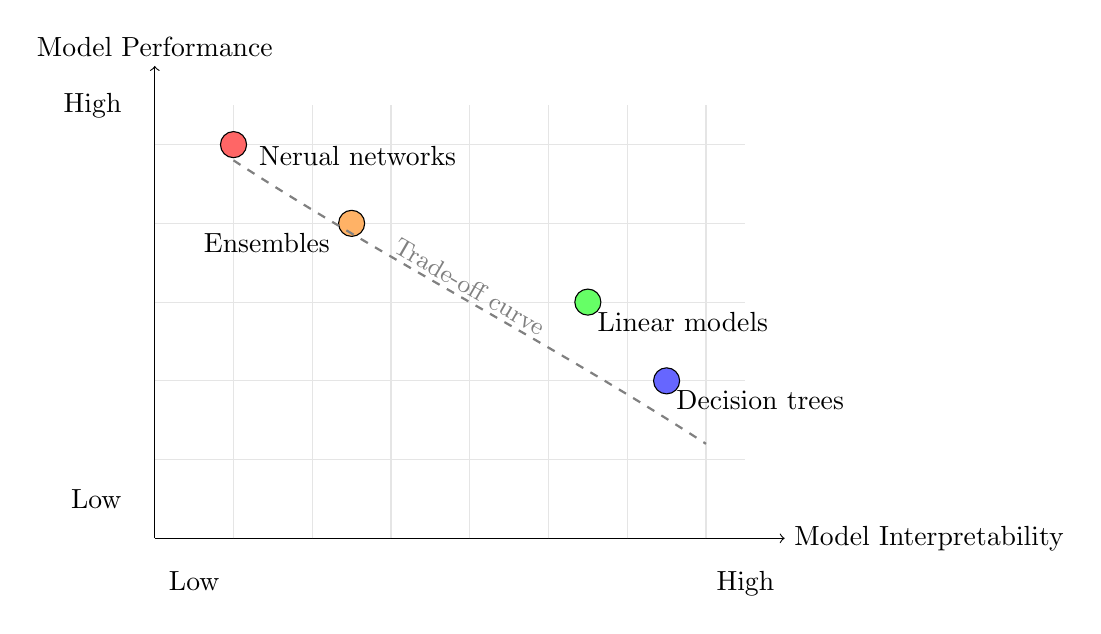
\begin{tikzpicture}
        % Define the axes
        \draw[->] (0,0) -- (8,0) node[right] {Model Interpretability};
        \draw[->] (0,0) -- (0,6) node[above] {Model Performance};
        
        % Add axis labels at the ends
        \node[below] at (0.5,-0.3) {Low};
        \node[below] at (7.5,-0.3) {High};
        \node[left] at (-0.3,0.5) {Low};
        \node[left] at (-0.3,5.5) {High};
        
        % Add grid lines (optional, subtle)
        \foreach \x in {1,2,...,7}
            \draw[gray!20] (\x,0) -- (\x,5.5);
        \foreach \y in {1,2,...,5}
            \draw[gray!20] (0,\y) -- (7.5,\y);
            
        % Position different model types
        % Deep Neural Networks (high performance, low interpretability)
        \node[circle, fill=red!60, draw, minimum size=8pt] at (1,5) {};
        \node[below right] at (1.2,5.1) {Nerual networks};
        
        % Ensemble Methods (medium-high performance, low-medium interpretability)
        \node[circle, fill=orange!60, draw, minimum size=8pt] at (2.5,4) {};
        \node[below right] at (0.5,4) {Ensembles};
        
        % Linear Models (medium performance, high interpretability)
        \node[circle, fill=green!60, draw, minimum size=8pt] at (5.5,3) {};
        \node[below right] at (5.5,3) {Linear models};
        
        % Decision Trees (medium-low performance, high interpretability)
        \node[circle, fill=blue!60, draw, minimum size=8pt] at (6.5,2) {};
        \node[below right] at (6.5,2) {Decision trees};
        

        
        % Add a general trend line (optional)
        \draw[dashed, thick, gray] (1,4.8) .. controls (3,3.5) and (5,2.5) .. (7,1.2);
        \node[gray, rotate=-30] at (4,3.2) {\small Trade-off curve};
        
    \end{tikzpicture}
    \caption{The interpretability-performance trade-off in machine learning. Different model classes are positioned according to their typical interpretability and performance characteristics. The dashed line illustrates the general trade-off between these two properties.}
    \label{fig:interpretability-performance-tradeoff}
\end{figure}

In Figure~\ref{fig:interpretability-performance-tradeoff} we present the popular trade-off between interpretability and performance of different model classes.

\section{Outline of the Thesis}

\begin{figure}[htbp]
    \centering
    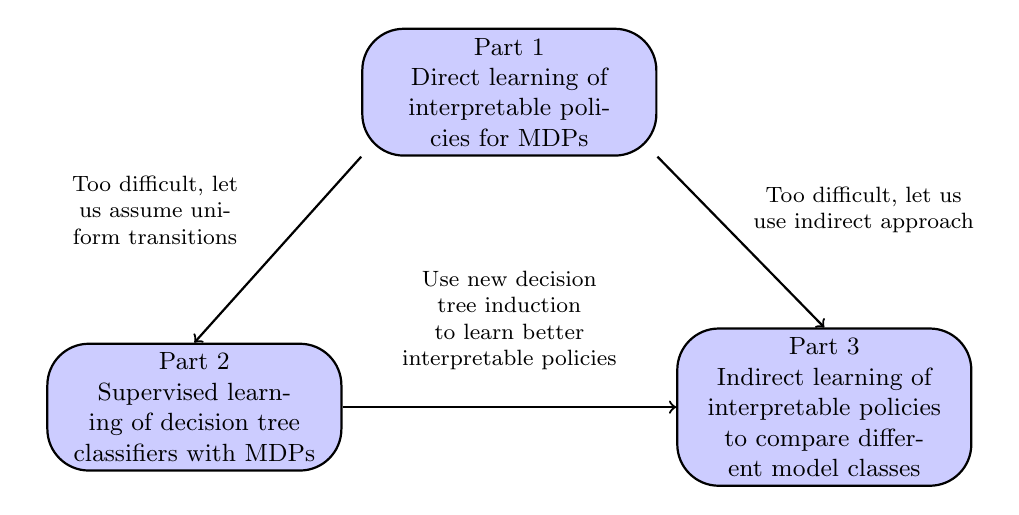
\begin{tikzpicture}[
        bubble/.style={rectangle, rounded corners=15pt, draw, thick, fill=blue!20, text width=3.5cm, text centered, minimum height=1.5cm, font=\small},
        arrow/.style={->, thick},
        label/.style={font=\footnotesize, text width=3cm, text centered}
    ]
        
        % Define the three vertices of the triangle
        % Top bubble - Chapter 1
        \node[bubble] (ch1) at (0,4) {Part 1\\Direct learning of interpretable policies for MDPs};
        
        % Bottom left bubble - Chapter 2  
        \node[bubble] (ch2) at (-4,0) {Part 2\\Supervised learning of decision tree classifiers with MDPs};
        
        % Bottom right bubble - Chapter 3
        \node[bubble] (ch3) at (4,0) {Part 3\\Indirect learning of interpretable policies to compare different model classes};
        
        % Arrow from Chapter 1 to Chapter 2
        \draw[arrow] (ch1.south west) -- (ch2.north);
        \node[label] at (-4.5,2.5) {Too difficult, let us assume uniform transitions};
        
        % Arrow from Chapter 1 to Chapter 3  
        \draw[arrow] (ch1.south east) -- (ch3.north);
        \node[label] at (4.5,2.5) {Too difficult, let us use indirect approach};

        % Arrow from Chapter 1 to Chapter 3  
        \draw[arrow] (ch2.east) -- (ch3.west);
        \node[label] at (0,1.1) {Use new decision tree induction to learn better interpretable policies};
        
        
    \end{tikzpicture}
    \caption{Thesis structure showing the progression from direct reinforcement learning of decision tree policies (Chapter 1) to simplified approaches: supervised learning with uniform transitions (Chapter 2) and indirect learning methods (Chapter 3).}
    \label{fig:thesis-outline}
\end{figure}
\section{Technical Preliminaries}
\subsection{What are decision trees?}
(figure)
As mentionned earlier, as opposed to neural networks, decision trees are supposidly very interpretable because the only apply boolean operations on the program input without relying on internal complex representations.
\begin{definition}[Decision tree]
A decision tree is a rooted tree $T = (V, E)$ where:
\begin{itemize}
\item Each internal node $v \in V$ is associated with a test function $f_v: \mathcal{X} \rightarrow \{0, 1\}$ that maps input features $x \in \mathcal{X}$ to a boolean.
\item Each edge $e \in E$ from an internal node corresponds to an outcome of the associated test function.
\item Each leaf node $\ell \in V$ is associated with a prediction $y_\ell \in \mathcal{Y}$, where $\mathcal{Y}$ is the output space.
\item For any input $x \in \mathcal{X}$, the tree defines a unique path from root to leaf, determining the prediction $T(x) = y_\ell$ where $\ell$ is the reached leaf.
\end{itemize}
\end{definition}
For non-sequential decision processes such as classification; it is possible to efficiently compute decision trees with induction over some training examples (cite). However 
\subsection{How to learn decision trees?}
\begin{figure}
    \centering
    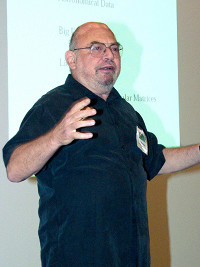
\includegraphics[width=0.3\textwidth]{images/images_intro/Leo_Breiman.jpg}
    \caption{The american statistician Leo Breiman (1928-2005) author of \textit{Classification and Regression Trees} (1984)}
\end{figure}
What about reinforcement learning?
\subsection{Markov decision processes/problems}
(figure)
Markov decision processes (MDPs) were first introduced in the 1950s by Richard Bellman (cite). Informally, an MDP models how an agent acts over time to achieve its goal. At every timestep, the agent observes its current state, e.g. a patient weight and tumor size, and takes an action, e.g. injects a certain amount of chemotherapy. When doing a certain action in a certain state, the agent gets a reward that helps it evaluate the quality of its action with respect to its goal, e.g., the tumor size decrease when the agent has to cure cancer. Finally, the agent is provided with a new state, e.g. the updated patient state, and repeats this process over time. Following Martin L. Puterman's book on MDPs (cite), we formally define as follows.
\begin{definition}[Markov decision process] An MDP is a tuple $\mathcal{M} = \langle S, A, R, T, T_0 \rangle$ where:
\begin{itemize}
\item $S$ is a finite set of states $s \in \mathbb{R}^n$ representing all possible configurations of the environment.
\item $A$ is a finite set of actions $a \in \mathbb{Z}^m$ available to the agent.
\item $R: S \times A \rightarrow \mathbb{R}$ is the reward function that assigns a real-valued reward to each state-action pair.
\item $T: S \times A \rightarrow \Delta(S)$ is the transition function that maps state-action pairs to probability distributions over next states, where $\Delta(S)$ denotes the probability simplex over $S$.
\item $T_0 \in \Delta(S)$ is the initial distribution over states.
\end{itemize}
\end{definition}
Now we can also model the ``goal'' of the agent. Informally, the goal of an agent is to behave such that it gets as much reward as it can over time. For example, in the cancer treatment case, the best reward the agent can get is to completely get rid of the patient's tumor after some time. Furthermore, we want our agent to prefer behaviour that gets rid of the patient's tumor as fast as possible. We can formally model the agent's goal as an optimization problem as follows. %talk about alignment?
\begin{definition}[Markov decision problem] Given an MDP $\mathcal{M}=\langle S, A, R, T, T_0 \rangle$, the goal of an agent following policy $\pi: S \rightarrow A$ is to maximize the expected discounted sum of rewards:
$$J(\pi) = \mathbb{E}\left[\sum_{t=0}^{\infty} \gamma^t R(s_t, a_t) \mid s_0 \sim T_0, a_t = \pi(s_t), s_{t+1} \sim T(s_t, a_t)\right]$$
where $\gamma \in (0,1)$ is the discount factor that controls the trade-off between immediate and future rewards.
\end{definition}
Hence, algorithms presented in this manuscript aim to find solutions to Markov decision problems, i.e. the optimal policy: $\pi^\star =\underset{\pi}{\operatorname{argmax}}J(\pi)$
For the rest of this text, we will use an abuse of notation and denote both a Markov decision process and the associated Markov decision problem by MDP.
\subsection{Exact solutions for Markov decision problems}
It is possible to compute the exact optimal policy $\pi^\star$ using dynamic programming (cite). Indeed, one can leverage the Markov property to find for all states the best action to take based on the reward of upcoming states.
\begin{definition}[Value of a state] The value of a state $s\in S$ under policy $\pi$ is the expected discounted sum of rewards starting from state $s$ and following policy $\pi$:
    $$V^\pi(s) = \mathbb{E}\left[\sum_{t=0}^{\infty} \gamma^t R(s_t, a_t) \mid s_0 = s, a_t = \pi(s_t), s_{t+1} \sim T(s_t, a_t)\right]$$
    Applying the Markov property gives a recursive definition of the value of $s$ under policy $\pi$:
    $$V^\pi(s) = R(s,\pi(s)) + \gamma \sum_{s' \in S} T^{s'}(s,\pi(s))V^\pi(s')$$
    where $T^{s'}(s,\pi(s))$ is the probability of transitioning to state $s'$ when taking action $\pi(s)$ in state $s$.
\end{definition}
\begin{definition}[Optimal value of a state] The optimal value of a state $s\in S$, $V^\star(s)$, is the value of state $s$ when following the optimal policy: $V^{\pi^{\star}}(s)$.
    $$V^{\star}(s) = V^{\pi^{\star}}(s) = \underset{\pi}{\max}\left[J(\pi)\right]$$
\end{definition}
Hence, the algorithms we study in the thesis can also be seen as solving the problem: $\pi^{\star} = \underset{\pi}{\operatorname{argmax}}\mathbb{E}\left[V^{\pi}(s_0)|s_0\sim T_0 \right]$. The well-known Value Iteration algorithm (algorithm) solves this problem exactly (cite). 

More realistically, neither the transition kernel $T$ nor the reward function $R$ of the MDP are known, e.g., the doctor can't \textbf{know} how the tumor and the patient health will change after a dose of chemotherapy, it can only \textbf{observe} the change. This distinction between the information available to the agent is paralleled with the distinction between dynamic programming and reinforcement learning (RL) that we describe next. 
\subsection{Reinforcement learning of approximate solutions to MDPs}
(figrure)
\begin{figure}
    \centering
    \begin{subfigure}[b]{0.22\textwidth}
        \centering
        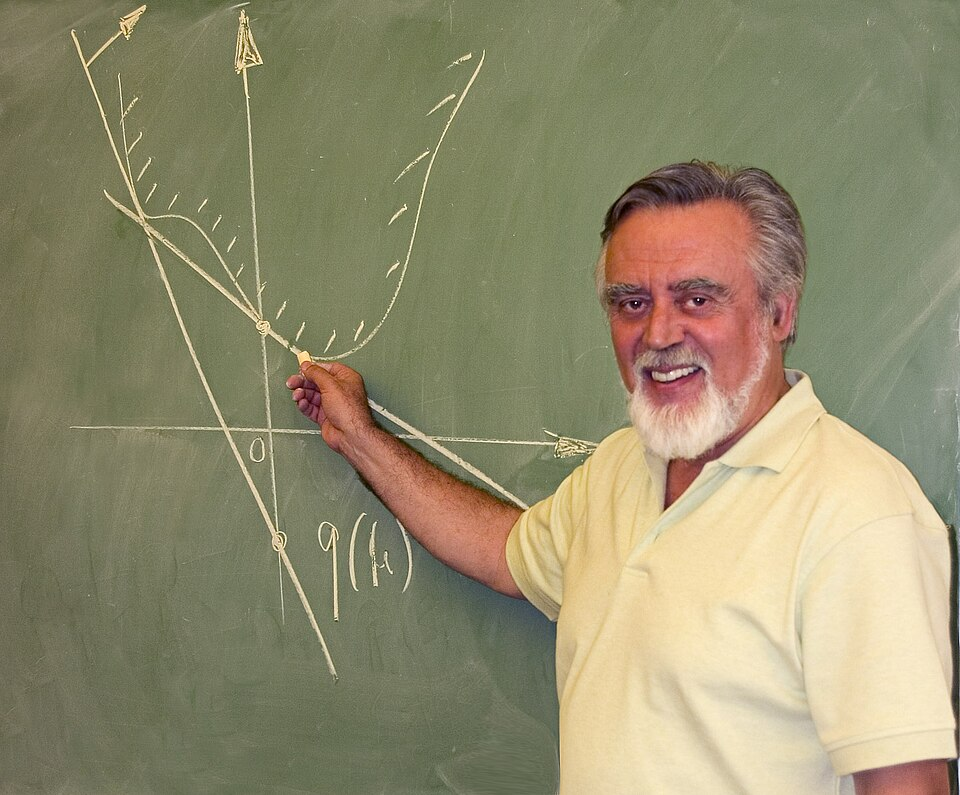
\includegraphics[width=\textwidth]{images/images_intro/Dimitri_Wiki_Pict.jpg}
        \caption{D. Bertsekas}
    \end{subfigure}
    \hfill
    \begin{subfigure}[b]{0.22\textwidth}
        \centering
        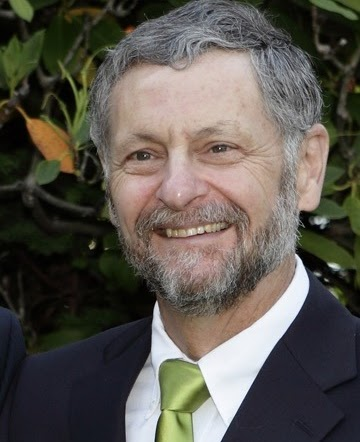
\includegraphics[width=\textwidth]{images/images_intro/puterman.jpg}
        \caption{M.L. Puterman}
    \end{subfigure}
    \hfill
    \begin{subfigure}[b]{0.22\textwidth}
        \centering
        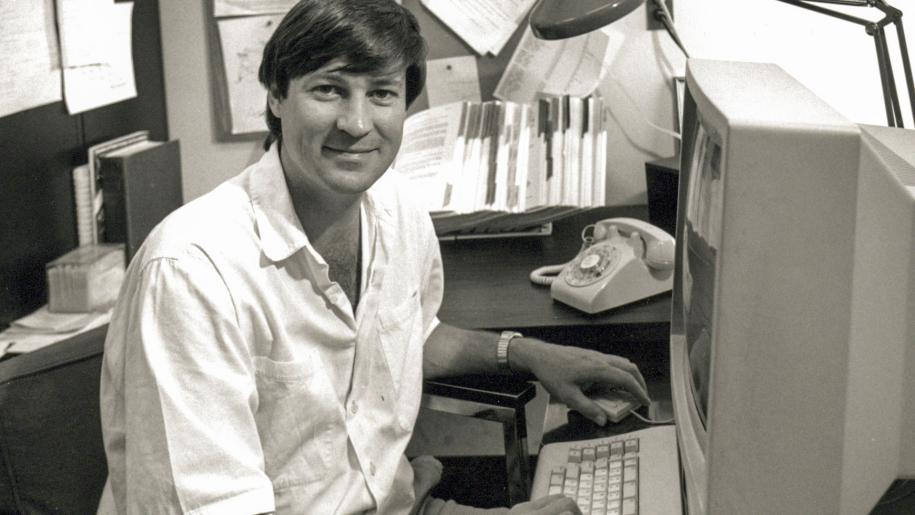
\includegraphics[width=\textwidth]{images/images_intro/Barto_1982_umass_amherst.jpg}
        \caption{A. Barto}
    \end{subfigure}
    \hfill
    \begin{subfigure}[b]{0.22\textwidth}
        \centering
        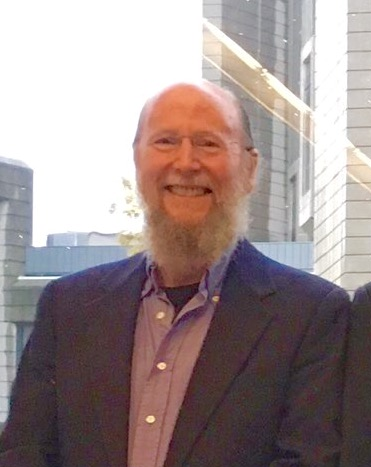
\includegraphics[width=\textwidth]{images/images_intro/sutton.jpg}
        \caption{R. Sutton}
    \end{subfigure}
       \caption{The godfathers of sequential decision making. Andrew Barto and Richard Sutton are the ACM Turing Prize 2024 laureate and share an advisor advisee relationship.}
       \label{fig:three graphs}
\end{figure}
Reinforcement learning algorithms popularized by Richard Sutton (figure) (cite) don't \textbf{compute} an optimal policy but rather \textbf{learn} an approximate one based on sequences of observations ${(s_t, a_t, r_t, s_{t+1})}_t$.
RL algorithms usually fall into two categories: value-based (cite) and policy gradient (cite). The first group of RL algorithms computes an appromiation of $V^{\star}$ using temporal different learning (algorithms) (cite). The other class of RL algorithms leverage the policy gradient theorem (algorithm) (cite) to approximate $\pi^{\star}$.
Both class of algorithms are known to converge to the optimal value or policy under some conditions (cite) and have known great successes in real-world appilcations (cite).
The books from Puterman, Bertsekas, Sutton and Barto, offer a great overview of MDPs and algorithm to solve them.
There are many other ways to learn policies such as simple random search (cite) or model-based reinforcement learning. However, not many algorithms consider the learning of policies that can be easily understood by humans which we discuss next and that is the core of this manuscript.

